\section{误差理论与数据处理}
\subsection{误差的基本性质与处理}
\subsubsection{随机误差}
当对同一个测量值进行多次的等精度重复测量时,可以得到一系列的不同的测量值,这些测量值多多少少都会存在误差,它们的出现是没有确定的规律的,但对于它们总体而言,却有统计的规律性\scite{3}。

当测量的数据中不包括有系统误差和粗大误差的时候,随机误差的分布可以是正态分布,也可以是其他分布,比如,均匀分布、三角形分布、$ \chi^2 $分布等,而大多数随机误差都服从正态分布。

假设被测量的真值为$ L_0 $,而测得值为$ l_i(i=1,2,...,n) $,则测量数据的随机误差$ \delta_i $为
\begin{equation}
	\delta_i=l_i-L_0
\end{equation}

正态分布的分布密度函数$ f(\delta) $与分布函数$ F(\delta) $为
\begin{equation}
	f(\delta)=\frac{1}{\sigma\sqrt{2\pi}}e^{-\delta^2/(2\sigma^2)}
\end{equation}
\begin{equation}
F(\delta)=\frac{1}{\sigma\sqrt{2\pi}}\int_{-\infty}^{\delta}e^{-\delta^2/(2\sigma^2)}d\delta
\end{equation}
式中:$ \sigma $为总体标准差,$ e $为自然对数底。
\begin{enumerate}
	\item \textbf{算术平均值}
	
	\qquad 在一系列的测量值中,被测量的$ n $个测得值的代数和除以$ n $而得的值称为算术平均值\scite{3}。设$ l_1,l_2,...,l_n $为$ n $次测量所得的值,则算术平均值$ \bar{x} $为
	\begin{equation}
	\bar{x}=\frac{l_1+l_2+...+l_n}{n}=\frac{1}{n}\sum_{i=1}^{n}l_i
	\end{equation}
	当测量次数无限大时,算术平均值被认为是最接近于真值的。
	\item \textbf{标准差}
	
	\qquad 单次测量的标准差是同一个被测量,在相同条件下,测量列$ l_1,l_2,...,l_n $中单次测量的标准差是表征同一被测量$ n $次测量结果分散性的参数,并按下式计算。
	\begin{equation}
	\sigma=\sqrt{\frac{\sum\limits_{i=1}^{n}(l_i-L_0)^2}{n}}=\sqrt{\frac{\sum\limits_{i=1}^{n}\delta_i^2}{n}}
	\end{equation}
	式中:$ n $为测量次数(应充分大);$ \delta_i $为第$ i $个测量值所对应的随机误差,即测量值与被测量值的真值之差。
	
	\qquad 对于标准差恒等的测量,把它定义为等精度测量,对于相同的测量条件下所做的重复测量均为等精度测量。反之,则属于不等精度测量。
	
	\qquad 对同一被测量,在相同测量条件下,进行有限次测量得测量列$ l_1,l_2,...,l_n $,则单次测量标准差的估计值为
	\begin{equation}
	s=\sqrt{\frac{\sum\limits_{i=1}^{n}v_i^2}{n-1}}
	\end{equation}
	这也被叫做贝塞尔公式。
	
	\qquad 算术平均值的标准差,算术平均值的标准差$ \bar{s} $是表示同一被测量的各个独立测量数据算术平均值分散的参数。
	\begin{equation}
	\bar{s}=\frac{s}{\sqrt{n}}
	\end{equation}
	\item \textbf{测量的极限误差}
	
	\qquad 单次测量的极限误差,根据概率论知识,已知正态分布曲线可得:
	\begin{equation} p=\int_{-\infty}^{+\infty}f(\delta)d\delta=\int_{-\infty}^{+\infty}\frac{1}{\sigma\sqrt{2\pi}}e^{-\frac{\delta^2}{2\sigma^2}}d\delta=1
	\end{equation}
	由此,误差落在区间$ [-\delta,+\delta] $之间的概率为:
	\begin{equation}
	p=\int_{-\delta}^{+\delta}f(\delta)d\delta=\int_{-\delta}^{+\delta}\frac{1}{\sigma\sqrt{2\pi}}e^{-\frac{\delta^2}{2\sigma^2}}d\delta
	\end{equation}
	将上式进行变量转换,设
	\begin{equation}
	t=\frac{\delta}{\sigma},dt=\frac{d\delta}{\sigma}
	\end{equation}
	经变换,上式成为
	\begin{equation}
	p=\frac{1}{\sqrt{2\pi}}\int_{-t}^{+t}e^{-\frac{t^2}{2}}dt=\frac{2}{\sqrt{2\pi}}\int_{0}^{+t}e^{-\frac{t^2}{2}}dt=2\Phi(t)
	\end{equation}\begin{equation}
	\Phi(t)=\frac{1}{\sqrt{2\pi}}\int_{0}^{+t}e^{-\frac{t^2}{2}}dt
	\end{equation}
	若某随机误差在$ \pm t\sigma $范围内出现的概率为$ 2\Phi(t) $,则超出的概率为
	\begin{equation}
	\alpha=1-2\Phi(t)
	\end{equation}
	不同的$ t $时超出$ |\delta| $的概率是不同的,取不同的$ t $值时,极限误差可用下式表示:
	\begin{equation}
	\delta_{lim}x=\pm t\delta
	\end{equation}
	\qquad 算术平均值的极限误差
	\begin{equation} \delta_{lim}\bar{x}=\pm t_a\sigma_{\bar{x}} \end{equation}
	式中:$ t_a $为置信系数;$ \alpha $为超出极限误差的概率;$ \sigma_{\bar{x}} $为$ n $次测量的算术平均值标准差。
	\item \textbf{权}
	
	\qquad 在等精度测量中,但是在不等精度测量中,各个测量值的可靠程度是不一样的,所以用权来说明测量的可靠程度\scite{3}。再根据算术平均值标准差以及测量的次数来确定权,假设同一测量量有$ m $组不等精度的测量结果,可表示为
	\begin{equation}
	p_1:p_2:...:p_m=\frac{1}{\sigma_{\bar{x_1}}^2}:\frac{1}{\sigma_{\bar{x_2}}^2}:...:\frac{1}{\sigma_{\bar{x_m}}^2}
	\end{equation}
	\item \textbf{加权算术平均值}
	
	\qquad 在对m组测量量进行不等精度的测量时,得到的结果是$ \bar{x_1},\bar{x_2},...,\bar{x_m} $,设相应的测量次数为$ n_1,n_2,...,n_m $,可以得出全部测量的算术平均值为
	\begin{equation}
	\bar{x}=\frac{\sum\limits_{i=1}^{m}p_i\bar{x}_i}{\sum\limits_{i=1}^{m}p_i}
	\end{equation}
	\item \textbf{加权算术平均值的标准差}
	\begin{equation}
	\bar{s}=\sqrt{\frac{\sum\limits_{i=1}^{m}p_iv_{\bar{x_i}}^2}{(m-1)\sum\limits_{i=1}^{m}p_i}}
	\end{equation}
\end{enumerate}
\subsubsection{系统误差}
\begin{enumerate}
	\item \textbf{系统误差的产生原因}
	
	\qquad 系统误差是由多方面因素引起的:测量装置方面,环境方面的因素,测量方法的因素,测量人员方面的因素。
	\item \textbf{系统误差的发现}
	
	\qquad 发现系统误差的方法有很多种,实验对比法、残余误差观察法、残余误差校核法、不同公式计算标准差法。
	\item \textbf{系统误差的减小与排除}
	
	\qquad 消除系统误差有两种方法,第一种是从产生误差根源上消除,第二种是用修正方法消除系统误差。常用的不变系统误差消除法有:代替法、抵消法、交换法。线性系统误差消除法有:对称法。周期性系统误差消除法有:半周期法。
\end{enumerate}
\subsubsection{粗大误差}
在一系列重复的测量数据中,如果有个别的数据(最大值或最小值)严重地偏离了它所属样本的其他数据,则可以怀疑该组数据中含有粗大误差。
\begin{enumerate}
	\item \textbf{粗大误差产生的原因}
	
	\qquad 产生粗大误差的原因是多方面的,不过大致可以归纳为测量人员的主观原因和客观外界条件的原因。
	\item \textbf{粗大误差的特点}
	
	\qquad 粗大误差的特点可以总结为以下三点,第一,在引起粗大误差的各种因素中,很难事先预测到,所以它具有突发性。第二,产生的粗大误差一般都远大于正常测量值之间的距离,所以它一般为较大的数值。第三,含有粗大误差的异常数据个数一般都很少,所以它有数量少的特点。
	\item \textbf{判别粗大误差的准则}
	
	\qquad 遇到粗大误差时,一定要慎重对待,并要根据判别准则予以确定。用来判别粗大误差的准则:$ 3\sigma $准则(莱以特准则)、罗曼诺夫斯基准则($ t $检验准则)、格拉布斯准则、狄克逊准则、奈尔准则、精细准则、肖维涅准则。
	
	\qquad 在这里主要介绍狄克逊准则,因为它不需要事先求出标准差$ \sigma $,而且在Matlab数据处理时会用到该方法检验粗大误差。狄克逊研究了$ x_1,x_2,...,x_n $的顺序统计量$ x_{(i)} $的分布,当$ x_{(i)} $服从正态分布时,得到$ x_{(i)} $的统计量
	\begin{equation}\begin{cases}
		r_{10}=\frac{x_{(n)}-x_{(n-1)}}{x_{(n)}-x_{(1)}}\\
		r_{11}=\frac{x_{(n)}-x_{(n-1)}}{x_{(n)}-x_{(2)}}\\
		r_{21}=\frac{x_{(n)}-x_{(n-2)}}{x_{(n)}-x_{(2)}}\\
		r_{22}=\frac{x_{(n)}-x_{(n-2)}}{x_{(n)}-x_{(3)}}
	\end{cases}\end{equation}
	的分布,选定显著度$ \alpha $,得到统计量的临界值$ r_0(n,\alpha) $,当测量值的统计值$ r_{ij} $大于临界值,则认为$ x_n $含有粗大误差。
	
	\qquad 统计量的临界值$ r_0(n,\alpha) $的查询见附录A 狄克逊检验统计量和临界值。
\end{enumerate}

\subsubsection{等精度测量数据的误差分析}
前面讨论了三类测量误差,它们的有各自的特点,因而处理的方法也有较大差别。等精度测量处理过程如图1-1所示,如下面等精度测量处理过程的例子。
\paragraph{例 } 对某一物体进行等精度测量9次,得到表1-1的数据(单位略),求测量结果。

\begin{figure}[H]
	\centering
	\captionsetup{type=table}
	\caption{\textbf{某9次等精度测量数据}}
	\begin{tabular}{|p{3cm}<{\centering}|p{3cm}<{\centering}|p{3cm}<{\centering}|p{3cm}<{\centering}|}
	\hline 
		序号	&  $ l $&  $ v_i $&  $ v_i^2 $\\	\hline 
		1&  24.774&  -0.001&  0.000001\\ \hline 
		2&  24.778&  +0.003&  0.000009\\ \hline 
		3&  24.771&  -0.004&  0.000016\\ \hline
		4&  24.780&  +0.005&  0.000025\\ \hline
		5&  24.772&  -0.003&  0.000009\\ \hline
		6&  24.777&  +0.002&  0.000004\\ \hline
		7&  24.773&  -0.002&  0.000004\\ \hline
		8&  24.775&		  0&  		 0\\ \hline
		9&  24.774&  -0.001&  0.000001\\ \hline
		\multicolumn{4}{|c|}{$ \sum\limits_{i=1}^{9}x_i=222.974,\quad\bar{x}=24.775,\quad\sum\limits_{i=1}^{9}v_i=-0.001,\quad\sum\limits_{i=1}^{9}v_i^2 =0.000069$}\\ \hline
	\end{tabular}
\end{figure}
\begin{figure}[H]
	\centering
	\begin{tikzpicture}[
	>=latex,
	node distance=5mm,
	hv path/.style={to path={-| (\tikztotarget)}},
	vh path/.style={to path={|- (\tikztotarget)}},
	startend/.style={draw,rectangle,rounded corners=2mm,minimum size = 6mm,	thick},
	ioput/.style={draw,trapezium,trapezium left angle=60, trapezium right angle=120,inner sep = 5pt},
	chuli/.style={draw,rectangle,minimum size=6mm,thick},
	panduan/.style={draw,diamond,minimum size=6mm,shape aspect=3,inner sep = 0.1pt,thick}
	]
	\node	(a)		[startend]				{开始};
	\node	(b)		[ioput,below=of a]		{导入测量数据$ l_i(i=1,2,...,n) $};
	\node	(c)		[panduan,below=of b]	{是否有粗大误差?};
	\node	(d)		[chuli,right=of c]		{剔除含有粗大误差数据};
	\node	(e)		[panduan,below=of c]	{是否有系统误差?};
	\node	(f)		[chuli,below=of e]		{计算算术平均值$ \bar{x} $};
	\node	(g)		[chuli,below=of f]		{修正算术平均值$ \bar{x}=\bar{x}+\Delta $};
	\node	(h)		[chuli,below=of g]		{计算单次测量的标准差$ s $};
	\node	(i)		[chuli,below=of h]		{计算算术平均值标准差$ s(\bar{x}) $};
	\node	(j)		[chuli,below=of i]		{根据显著性水平及分布查表得$ t_\alpha $};
	\node	(k)		[chuli,below=of j]		{计算算术平均值极限误差$ \delta_{lim}\bar{x}=\pm t_\alpha s(\bar{x}) $};
	\node	(l)		[chuli,below=of k]		{给出测量结果$ L=\bar{x}+\delta_{lim}\bar{x} $};
	\node	(m)		[startend,below=of l]	{结束};
	
	\draw[->](a)--(b);
	\draw[->](b)--(c);
	\draw[->](c)--(d);
	\path (d.north) edge [->,vh path]($(b.south)!.5!(c.north)$);
	\draw[->](c)--(e);
	\draw[->](e)--(f);
	\draw[->](f)--(g);
	\draw[->](g)--(h);
	\draw[->](h)--(i);
	\draw[->](i)--(j);
	\draw[->](j)--(k);
	\draw[->](k)--(l);
	\draw[->](l)--(m);
	
	\node at (0.25,-3.6){否};
	\node at (2.15,-2.5){是};
	\end{tikzpicture}
	\caption{\textbf{等精度测量数据处理流程图}}
\end{figure}
\begin{enumerate}
	\item \textbf{粗大误差判别(用狄克逊准则差别)}
	
	将数据进行从小到大排序,可以得到最小值$ x_{(1)} $和最大值$ x_{(9)} $。
	\begin{equation} x_{(1)}=24.771,x{(9)}=24.780 \end{equation}
	首先判断最大值$ x_{(9)} $,因$ n=9 $,帮计算得统计量$ r_{11} $为
	\begin{equation}
	r_{11}=\frac{x_{(9)}-x_{(8)}}{x_{(9)}-x_{(2)}}=\frac{24.780-24.778}{24.780-24.772}=\frac{0.002}{0.008}=0.400
	\end{equation}
	查狄克逊准则临界表\footnote{见附录A}可知\begin{equation} r_0(9,0.05)=0.512 \end{equation}
	\begin{equation} r_{11}=0.4<r_0(9,0.05)=0.512 \end{equation}
	可以判断最大值$ x_{(9)} $不含有粗大误差,再对最小值$ x_{(1)} $计算相应统计量$ r'_{11} $
	\begin{equation}
	r'_{11}=\frac{x_{(1)}-x_{(2)}}{x_{(1)}-x_{(8)}}=\frac{24.771-24.772}{24.771-24.778}=\frac{-0.001}{-0.005}=0.167
	\end{equation}
	\begin{equation} r'_{11}=0.167<r_0(9,0.05)=0.512 \end{equation}
	可以判断最小值$ x_{(1)} $不含有粗大误差,故可以判断该测量数据不含有粗大误差。
	\item \textbf{系统误差差别(用残余误差观察法)}
	
	\qquad 如图1-2所示,发现残余误差大体相同,无明显变化规律,可以认为不存在系统误差。
	\begin{figure}[H]
		\centering
		\begin{tikzpicture}
			\begin{axis}[ymajorgrids,minor tick num=1,width=15cm,height=7cm]
				\addplot[only marks] coordinates {
					(1,-0.001)
					(2,0.003)
					(3,-0.004)
					(4,0.005)
					(5,-0.003)
					(6,0.002)
					(7,-0.002)
					(8,0)
					(9,-0.001)
				};
			\end{axis}
		\end{tikzpicture}
		\caption{\textbf{残余误差分布}}
	\end{figure}

	\item \textbf{随机误差处理}
		\begin{enumerate}
			\item 求算术平均值:
			\begin{equation}\bar{x}=\frac{\sum\limits_{i=1}^{n}l_i}{n}=\frac{222.974}{9}mm=24.7749mm\approx24.775mm\end{equation}
			\item 求残余误差(见列表):\begin{equation}v_i=l_i-\bar{x}\end{equation}
			\item 校核算术平均值和残余误差。\begin{equation} \left| \sum\limits_{i=1}^{9}v_i \right|=0.001mm<\left(\frac{n}{2}-0.5\right)A=4\times0.001mm=0.004mm  \end{equation}
			以上计算正确,否则,应重新进行计算和校核:
			\item 求单次测量的标准差(贝塞尔公式)\begin{equation} s=\sqrt{\frac{\sum\limits_{i=1}^{n}v_i^2}{n-1}}=\sqrt{\frac{0.000069}{8}mm^2}=0.0029mm \end{equation}
			\item 求算术平均值的标准差:\begin{equation} \bar{s}=\frac{s}{\sqrt{n}}\approx0.001mm \end{equation}
			\item 求算术平均值的极限误差。
			
			\qquad 因为测量的次数较少,算术平均值的极限误差按$ t $分布计算,已知$ v=n-1=8 $,取$ \alpha=0.05 $查得$ t $分布临界值表得$ t_\alpha=2.31 $,则算术平均值的极限误差$ \delta_{lim}\bar{x} $为\begin{equation} \delta_{lim}\bar{x}=\pm t_\alpha\sigma_{\bar{x}}=\pm2.31\times0.001mm=\pm0.0023mm \end{equation}
		\end{enumerate}
	\item \textbf{测量结果}\begin{equation} L=\bar{x}\pm\delta_{lim}\bar{x}=(24.755\pm0.0023)mm \end{equation}
\end{enumerate}
\subsubsection{不等精度测量数据的误差分析}
\begin{figure}[H]
	\centering
	\begin{tikzpicture}[
	>=latex,
	node distance=5mm,
	hv path/.style={to path={-| (\tikztotarget)}},
	vh path/.style={to path={|- (\tikztotarget)}},
	startend/.style={draw,rectangle,rounded corners=2mm,minimum size = 6mm,	thick},
	ioput/.style={draw,trapezium,trapezium left angle=60, trapezium right angle=120,inner sep = 5pt},
	chuli/.style={draw,rectangle,minimum size=6mm,thick},
	panduan/.style={draw,diamond,minimum size=6mm,shape aspect=3,inner sep = 0.1pt,thick}
	]
	\node	(a)		[startend]				{开始};
	\node	(b)		[ioput,below=of a]		{导入测量数据$ L_i(i=1,2,...,m) $};
	\node at (-4,-2.4)	(cl)	[chuli]		{计算算术平均值$ \bar{x_1} $};
	\node at (4,-2.4)	(cr)	[chuli]		{计算算术平均值$ \bar{x_m} $};
	\node	(dl)	[panduan,below=of cl]	{是否有粗大误差?};
	\node	(dr)	[panduan,below=of cr]	{是否有粗大误差?};
	\node	(el)	[chuli,right=of dl,align=center]		{剔除含有粗\\大误差数据};
	\node	(er)	[chuli,right=of dr,align=center]		{剔除含有粗\\大误差数据};
	\node	(fl)	[panduan,below=of dl]	{是否有系统误差?};
	\node	(fr)	[panduan,below=of dr]	{是否有系统误差?};
	\node	(gl)	[chuli,below=of fl]		{修正算术平均值$ \bar{x_1}=\bar{x_1}+\Delta_1 $};
	\node	(gr)	[chuli,below=of fr]		{修正算术平均值$ \bar{x_m}=\bar{x_m}+\Delta_m $};
	\node	(hl)	[chuli,below=of gl]		{计算单次测量的标准差$ s_1 $};
	\node	(hr)	[chuli,below=of gr]		{计算单次测量的标准差$ s_m $};
	\node	(il)	[chuli,below=of hl]		{计算加权算术平均值标准差$ s(\bar{x_1}) $};
	\node	(ir)	[chuli,below=of hr]		{计算加权算术平均值标准差$ s(\bar{x_m}) $};
	\node	(jl)	[chuli,below=of il]		{计算相应的权$ p_1=1/(s(\bar{x_1}))^2 $};
	\node	(jr)	[chuli,below=of ir]		{计算相应的权$ p_m=1/(s(\bar{x_m}))^2 $};
	\node at (0,-12)	(k)		[chuli]		{计算加权算术平均值$ \bar{x}=\frac{\sum\limits_{i=1}^{m}p_i\bar{x_i}}{\sum\limits_{i=1}^{m}p_i} $};
	\node	(l)		[chuli,below=of k]		{计算加权算术平均值标准差$ \bar{s}=\bar{s_i}\sqrt{\frac{p_i}{\sum\limits_{i=1}^{m}p_i}} $};
	\node	(m)		[chuli,below=of l]		{计算加权算术平均值极限误差$ \delta_{lim}\bar{x}=\pm t_\alpha s(\bar{x}) $};
	\node	(n)		[chuli,below=of m]		{给出测量结果$ L=\bar{x}+\delta_{lim}\bar{x} $};
	\node	(o)		[startend,below=of n]	{结束};

	\draw[->](a)--(b);
	\path (b) edge [->,hv path](cl);
	\path (b) edge [->,hv path](cr);
	\draw[->](cl)--(dl);\draw[->](cr)--(dr);
	\draw[->](dl)--(el);\draw[->](dr)--(er);
	\path (el) edge [->,vh path](cl);
	\path (er) edge [->,vh path](cr);
	\draw[->](dl)--(fl);\draw[->](dr)--(fr);
	\draw[->](fl)--(gl);\draw[->](fr)--(gr);
	\draw[->](gl)--(hl);\draw[->](gr)--(hr);
	\draw[->](hl)--(il);\draw[->](hr)--(ir);
	\draw[->](il)--(jl);\draw[->](ir)--(jr);
	\path (jl) edge [->,vh path](k);
	\path (jr) edge [->,vh path](k);
	\draw[->](k)--(l);
	\draw[->](l)--(m);
	\draw[->](m)--(n);
	\draw[->](n)--(o);

	\node at (-1.9,-3.6){是};
	\node at (6.1,-3.6){是};
	\node at (-3.8,-4.8){否};
	\node at (4.2,-4.8){否};
	\node at (-3.8,-6.6){是};
	\node at (4.2,-6.6){是};
	\end{tikzpicture}
	\caption{\textbf{不等精度测量数据处理流程图}}
\end{figure}
\paragraph{例}对某一角度进行6组不等精度的测量,假设不含有随机误差和系统误差,各组测量的数据如下:

测6次得$ \alpha_1=75^\circ18'16'' $,测30次得$ \alpha_2=75^\circ18'10'' $,测24次得$ \alpha_3=75^\circ18'08'' $,测12次得$ \alpha_4=75^\circ18'16'' $,测12次得$ \alpha_5=75^\circ18'13'' $,测36次得$ \alpha_6=75^\circ18'09'' $,求得最后的测量结果。
\begin{enumerate}
	\item 根据测量的数据求出各组的权,有\begin{equation} p_1:p_2:p_3:p_4:p_5:p_6=1:5:4:2:2:6 \end{equation}取\begin{equation} p_1=1,p_2=5,p_3=4,p_4=2,p_5=2,p_6=6 \end{equation}
	\item 求出加权算术平均值$ \bar{\alpha} $:\begin{equation} \bar{\alpha}=\sum_{i=1}^{6}p_i\alpha_i=75^\circ18'10'' \end{equation}
	\item 求残余误差,由公式$ v_i=\alpha_i-\bar{\alpha} $得\begin{equation} v_1=-4'',v_2=0,v_3=-2'',v_4=6'',v_5=3'',v_6=-1'' \end{equation}
	\item 校核算术平均值及残余误差。用加权残余误差代数和等于0来校核。因:\begin{equation} \sum_{i=1}^{6}p_iv_i=0 \end{equation}所以计算正确。
	\item 求加权算术平均值的标准差:\begin{equation} \bar{s}=\sqrt{\frac{\sum\limits_{i=1}^{6}p_iv_i^2}{(m-1)\sum\limits_{i=1}^{6}p_i}}=1.1'' \end{equation}
	\item 求加权算术平均值的极限误差,可以根据测量数据得出,该数据服从正态分布,取置信系数$ t=3 $,则极限误差为\begin{equation} \delta_{lim}\bar{\alpha}=\pm3\bar{s}=\pm3.3'' \end{equation}
	\item 测量结果为\begin{equation} \alpha=\bar{\alpha}+\delta_{lim}\bar{\alpha}=75^\circ18'10''\pm3.3'' \end{equation}
\end{enumerate}
\subsection{误差的合成}
前面讨论的都是直接测量的误差计算,可是在许多情况下,并不能对被测对象进行直接地测量,或者直接测量不能满足精度上的需要,需要采用间接测量。间接测量误差是各个直接测量值误差的函数,称这种误差为函数误差\footnote{《误差理论与数据处理》第79页函数误差的定义,详情见参考文献[1]}。其实就是研究误差的传递问题,对于这种有确定关系的误差计算,也中叫做误差的合成。

间接测量的数学模型为\begin{equation} y=f(x_1,x_2,...,x_n) \end{equation}
式中:$ x_1,x_2,...,x_n $为直接测量值,$ y $为间接测量值。

函数$ y $的全微分表达式为\begin{equation} dy=\frac{\partial f}{\partial x_1}dx_1+\frac{\partial f}{\partial x_2}dx_2+...+\frac{\partial f}{\partial x_n}dx_n \end{equation}
\subsubsection{系统误差的合成}
已定系统误差的合成,已定系统误差是指误差大小和方向均已确定的系统误差。在测量过程中,若有$ r $个已定系统误差,其误差分别为$ \Delta_1,\Delta_2,...,\Delta_r $,相应的误差传递函数为$ a_1,a_2,...,a_r $,则按代数和进行合成,求得总的系统误差为\begin{equation} \Delta=\sum_{i=1}^{r}a_i\Delta i \end{equation}

未定系统误差的合成,采用随机误差的合成公式。
\begin{enumerate}
	\item \textbf{标准差的合成}
	
	\qquad 当测量的过程中有$ s $个单项的未定系统误差,标准差分别为$ u_1,u_2,...,u_s $,相应的误差传递系数为$ a_1,a_2,...,a_s $,则合成后未定系统误差的总标准差为\begin{equation} u=\sqrt{\sum_{i=1}^{s}(a_iu_i)^2+2\sum_{1\leq i\leq j}^{s}\rho_{ij}a_ia_ju_iu_j} \end{equation}
	当$ \rho_{ij}=0 $时,则有\begin{equation} u=\sqrt{\sum_{i=1}^{s}(a_iu_i)^2} \end{equation}
	\item \textbf{极限误差的合成}
	
	\qquad 因为极限误差为$ e_i=\pm t_iu_i,i=1,2,...,s $,总的极限误差为$ e=\pm tu $,则可得\begin{equation} e=\pm t\sqrt{\sum_{i=1}^{s}(a_iu_i)^2+2\sum_{1\leq i\leq j}^{s}\rho_{ij}a_ia_ju_iu_j} \end{equation}
	当各个单项未定系统误差均服从正态分布,且$ \rho_{ij}=0 $时,则简化为\begin{equation} e=\pm\sqrt{\sum_{i=1}^{s}(a_ie_i)^2} \end{equation}
\end{enumerate}
\subsubsection{随机误差的合成}
\begin{enumerate}
	\item \textbf{标准差的合成}
	
	\qquad 若有$ q $个单项随机误差,它们的标准差分别为$ \sigma_1,\sigma_2,...,\sigma_q $其相应的误差传递函数为$ a_1,a_2,...,a_q $。合成的总标准差为\begin{equation} \sigma=\sqrt{\sum_{i=1}^{q}(a_i\sigma_i)^2+2\sum_{1\leq i<j}^{q}\rho_{ij}a_ia_j\sigma_i\sigma_j} \end{equation}
	
	\qquad 当相关系数$ \rho_{ij}=0 $,则有\begin{equation} \sigma=\sqrt{\sum_{i=1}^{q}(a_i\sigma_i)^2} \end{equation}
	\item \textbf{极限误差的合成}
	
	\qquad  已知各单项极限误差为$ \delta_1,\delta_2,...,\delta_q $,且置信概率相同,则总极限误差为\begin{equation} \delta=\pm\sqrt{\sum_{i=1}^{q}(a_i\delta_i)^2+2\sum_{1\le i<j}^{q}\rho_{ij}a_ia_j\delta_i\delta_j} \end{equation}
	式中:$ a_i $为各极限误差传递系数;$ \rho_{ij} $为任意误差间的相关系数。
	
	\qquad 引入置信系数后得:\begin{equation} \delta=\pm t\sqrt{\sum_{i=1}^{q}(a_i\delta_i)^2+2\sum_{1\le i<j}^{q}\rho_{ij}a_ia_j\delta_i\delta_j} \end{equation}
\end{enumerate}

\subsection{测量不确定度}
\subsubsection{标准不确定度的A类评定}
当被测量$ Y $取决于它$ N $个量$ X_1,X_2,...,X_N $时,则$ Y $的估计值$ y $的标准不确守度将取决于$ X_i $的估计值$ x_i $的标准不确定度$ u_{x_i} $,为此要先评定$ x_i $的标准不确定度$ u_{x_i} $,在其他$ X_j(j\neq i) $保持不变的情况下,仅对$ X_i $进行$ n $次等精度独立测量,用统计法由$ n $个观测值求得单次测量标准差$ \sigma_i $,则$ x_i $的标准不确定度$ u_{x_i} $的数值为\begin{equation} u_{x_i}=\frac{\sigma_i}{\sqrt{n}} \end{equation}
\subsubsection{标准不确定度的B类评定}
\begin{enumerate}
	\item 当测量估计值$ x $为正态分布时,由所取置信概率$ P $的分布区间半宽$ a $与包含因子$ k_p $来估计标准不确定度,即\begin{equation} u_x=\frac{a}{k_p} \end{equation}
	式中包含因子$ k_p $的数值由正态分布积分表查得。
	\item 当估计值$ x $取自相关资料,所给出的测量不确定度$ U_x $为标准差的$ k $倍时,则标准不确定度为\begin{equation} u_x=\frac{U_x}{k} \end{equation}
	\item 若已知估计值$ x $落在区间$ (x-a,x+a) $内的概率为1,且$ x $服从均匀分布,标准不确定度为\begin{equation} u_x=\frac{a}{\sqrt{3}} \end{equation}
	\item 当$ x $服从在区间$ (x-a,x+a) $内的三角分布,标准不确定度为\begin{equation} u_x=\frac{a}{\sqrt{6}} \end{equation}
	\item 当$ x $服从在区间$ (x-a,x+a) $内的反正弦分布,标准不确定度为\begin{equation} u_x=\frac{a}{\sqrt{2}} \end{equation}
\end{enumerate}
\subsubsection{自由度的确定}
\begin{enumerate}
	\item 对于标准不确定度A类评定的自由度,如果用贝塞尔计算的标准差,其自由度为 $ v=n-1 $,而用其他方法计算的标准差,自由度有所不同。
	\item 对于标准不确定度B类评定的自由度,由估计$ u $的相对标准差来确定,定义为\begin{equation} v=\frac{1}{2(\frac{\sigma_u}{u})^2} \end{equation}
	式中:$ \delta_u $为评定$ u $的标准差,$ \sigma_u/u $为评定$ u $的相对标准差。
\end{enumerate}
\subsubsection{测量不确定度合成}
\begin{enumerate}
	\item 合成标准不确定度\begin{equation} u_c=\sqrt{\sum_{i=1}^{n}u_i^2+2\sum_{1\le i<j}^{N}\rho_{ij}u_iu_j} \end{equation}
	其测量结果表示为\begin{equation} Y=y\pm u_c \end{equation}
	\item 展伸不确定度,它由合成标准不确定度$ u_c $乘以包含因子$ k $得到,即\begin{equation} U=ku_c \end{equation}
	其测量结果为\begin{equation} Y=y\pm U \end{equation}
\end{enumerate}
当各不确定度分量$ u_i $相互独立时,合成标准不确定度的自由度$ v $为\begin{equation} v=\frac{u_c^4}{\sum\limits_{i=1}^{N}\frac{u_i^4}{v_i}} \end{equation}
\subsection{最小二乘法处理}
测量结果的最可信赖值应使残余误差平方和最小(不等精度测量时,使加权残余误差平方和最小),这就是最小二乘法原理\footnote{《误差理论与数据处理》第125页最小二乘法的定义,详情见参考文献[1]}。
\begin{enumerate}
\item \textbf{等精度测量线性参数最小二乘法处理的正规方程}
\begin{figure}[H]
	\centering
	\begin{tikzpicture}[
	>=latex,
	node distance=5mm,
	chuli/.style={draw,rectangle,minimum size=6mm,thick}
	]

	\node	(a)	[chuli]								{根据具体问题列出误差方程};
	\node	(b)	[chuli,below=of a,align=center]		{按最小二乘法原理,利用函数求极值\\的方法将误差方程转换为正规方程};
	\node	(c)	[chuli,below=of b]					{求解正规方程,得到待求的估计量};
	\node	(d)	[chuli,below=of c]					{给出估计量的不确定度评定};
	
	\draw[->](a)--(b);
	\draw[->](b)--(c);
	\draw[->](c)--(d);

	\end{tikzpicture}
	\caption{\textbf{线性参数最小二乘法处理流程图}}
\end{figure}
线性参数的误差方程式为
\begin{equation} \begin{cases}
	v_1 = l_1-(a_{11}x_1+a_{12}x_2+...+a_{1t}x_t)\\
	v_2 = l_2-(a_{21}x_1+a_{22}x_2+...+a_{2t}x_t)\\
	\qquad \vdots\\
	v_n = l_n-(a_{n1}x_1+a_{n2}x_2+...+a_{nt}x_t)\\
\end{cases} \end{equation}
在等精度测量中,最小二乘条件式为\begin{equation} \sum_{i=1}^{n}v_i^2=v_1^2+v_2^2+...+v_n^2=min \end{equation}
经过转换和简化正规方程可写成
\begin{equation} \begin{cases}
	a_{11}v_1+a_{21}v_2+...+a_{n1}v_n=0\\
	a_{12}v_1+a_{22}v_2+...+a_{n2}v_n=0\\
	\qquad \vdots\\
	a_{1t}v_1+a_{2t}v_2+...+a_{nt}v_n=0
\end{cases} \end{equation}
转换为矩阵形式:
\begin{equation} \begin{bmatrix}
	a_{11}&a_{21}&\dots&a_{n1}\\
	a_{12}&a_{22}&\dots&a_{n2}\\
		  & 	 &\vdots\\
	a_{1t}&a_{2t}&\dots&a_{nt}
\end{bmatrix}\begin{bmatrix}
	v_1\\v_2\\\vdots\\v_n
\end{bmatrix}=\begin{bmatrix}
	0\\0\\\vdots\\0
\end{bmatrix} \end{equation}
即\begin{equation} A^TV=0 \end{equation}
这是等精度测量情况下矩阵形式表示的正规方程。
又因为\begin{equation} V=L-A\hat{X} \end{equation}
所以正规方程可写为\begin{equation} A^TL-A^TA\hat{X}=0 \end{equation}\begin{equation} (A^TA)\hat{X}=A^TL \end{equation}
令$ C=A^TA $,则方程为\begin{equation} C\hat{X}=A^TL \end{equation}
当矩阵$ C $满秩,可化为\begin{equation} \hat{X}=C^{-1}A^TL \end{equation}
得到$ \hat{X} $的数学期望为\begin{equation} E[\hat{X}]=E(C^{-1}A^TL)=C^{-1}A^TE(L)=C^{-1}A^TY=C^{-1}A^TAX=X \end{equation}
式中:$ Y,X $为列向量($ n\times1 $阶矩阵和$ t\times1 $阶矩阵)
\begin{equation} Y=\begin{bmatrix}
	Y_1\\Y_2\\\vdots\\Y_n
\end{bmatrix},X=\begin{bmatrix}
	X_1\\X_2\\\vdots\\X_t
\end{bmatrix} \end{equation}
\item \textbf{不等精度测量线性参数最小二乘法处理的正规方程}

	\qquad 不等精度测量时线性参数的误差方程和等精度的一样,只是条件式要取加权残余误差平方和最小,即\begin{equation} Z=\sum_{i=1}^{n}p_iv_i^2=min \end{equation}
	对$ Z $求导数并令其为0,最后求得正规方程为\begin{equation} \begin{cases}
		p_1a_{11}v_1+p_2a_{21}v_2+...+p_na_{n1}v_n=0\\
		p_1a_{12}v_1+p_2a_{22}v_2+...+p_na_{n2}v_n=0\\
		\qquad \vdots\\
		p_1a_{1t}v_1+p_2a_{2t}v_2+...+p_na_{nt}v_n=0
	\end{cases} \end{equation}
	用矩阵表示为\begin{equation} \begin{bmatrix}
		a_{11}&a_{21}&\dots&a_{n1}\\
		a_{12}&a_{22}&\dots&a_{n2}\\
		& 	 &\vdots\\
		a_{1t}&a_{2t}&\dots&a_{nt}
	\end{bmatrix}\begin{bmatrix}
		p_1	&	0	&	\dots&	0\\
		0	&	p_2	&	\dots&	0\\
		& 	 &\vdots\\
		0	&	0	&	\dots&	p_n
	\end{bmatrix}\begin{bmatrix}
		v_1\\v_2\\\vdots\\v_n
	\end{bmatrix}=\begin{bmatrix}
		0\\0\\\vdots\\0
	\end{bmatrix} \end{equation}
	即\begin{equation} A^TPV=0 \end{equation}
	而$ V=L-A\hat{X} $,所以\begin{equation} A^TP(L-A\hat{X})=0 \end{equation}
	由$ A^TPA\hat{X}=A^TPL $得出解为\begin{equation} \hat{X}=(A^TPA)^{-1}A^TPL \end{equation}
	令$ C^*=A^TPA $则\begin{equation} \hat{X}=(C)^{*-1}A^TPL \end{equation}
	这就是不等精度测量时,线性参数的最小二乘法处理。
	\begin{equation} E(\hat{X})=E((C)^{*-1}A^TPL)=(C)^{*-1}A^TPE(L)=(C)^{*-1}A^TPAX=X \end{equation}
	可见$ \hat{X} $是$ X $的无偏估计。
\end{enumerate}
\subsection{回归分析}
在生产科学中,还有另一类问题,即测量与数据处理的目的并不在于被测的估计值,而是为了找出两个变量或多个变量之间的内在关系,表达变量之间关系的方法有多种,比如散点图、表格、曲线、数学表达式等,其中数学表达式能较客观地反映事物的内在规律性。对此,要用到回归分析。

假设测量某导线在一定温度下$ x $下的电阻值$ y $得结果如表2所示(单位略),试找出它们之间的内在关系。
\begin{figure}[H]
	\centering
	\captionsetup{type=table}
	\caption{\textbf{某导线测量数据}}
	\begin{tabular}{|*{8}{p{1.5cm}<{\centering}|}}
			\hline 
			$ x $&  19.1&  25.0&  30.1&  36.0&  40.0&  46.5&  50.0\\\hline 
			$ y $&  76.30&  77.80&  79.75&  80.80&  82.35&  83.90&  85.10\\\hline 
	\end{tabular}
\end{figure}
为了研究电阻$ y $与温度$ x $之间的关系,把数据点画在坐标上,如图5所示。
\begin{figure}[H]
	\centering
	\begin{tikzpicture}
	\begin{axis}[minor tick num=1,width=10cm,height=8cm,xlabel=$ x $,ylabel=$ y $]
	\addplot[only marks] coordinates {
		(19.1,76.30)
		(25.0,77.80)
		(30.1,79.75)
		(36.0,80.80)
		(40.0,82.35)
		(46.5,83.90)
		(50.0,85.10)
	};
	\end{axis}
	\end{tikzpicture}
	\caption{\textbf{电阻与温度关系散点图}}
\end{figure}
设$ b_0 $和$ b $分别是$ y_t=\beta_0+\beta x_t+\varepsilon_t,t=1,2,...,N $的最小二乘估计,得到一元线性回归的回归方程为\begin{equation} \hat{y}=b_0+bx \end{equation}
应用最小二乘法求解回归系数,求得方程为\begin{equation} y=70.90+0.2824x \end{equation}
作出回归方程函数图对比,如图6。
\begin{figure}[H]
	\centering
	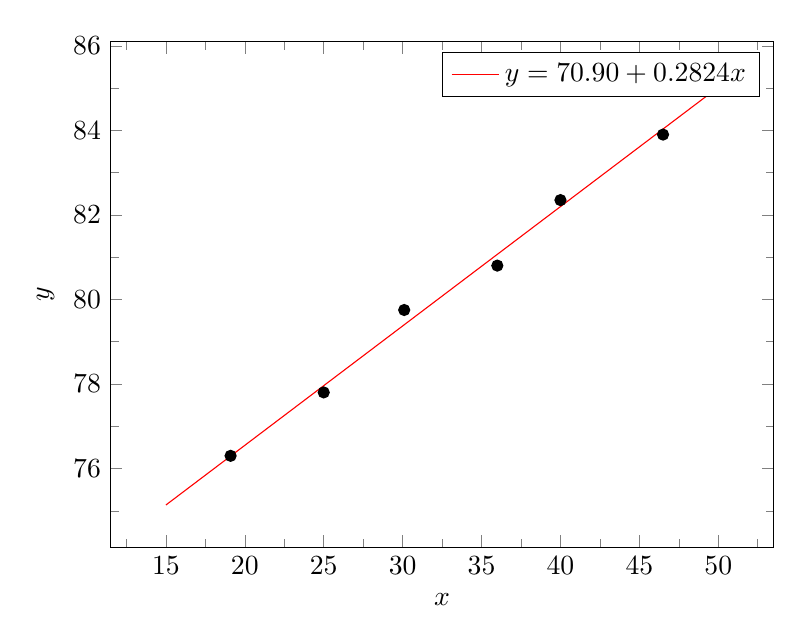
\begin{tikzpicture}
	\begin{axis}[minor tick num=1,width=10cm,height=8cm,xlabel=$ x $,ylabel=$ y $]
	\addplot[domain=15:50,samples=100, color=red,]{0.2824*x+70.90};
	\addlegendentry{$y=70.90+0.2824x$}
	\addplot[only marks] coordinates {
		(19.1,76.30)
		(25.0,77.80)
		(30.1,79.75)
		(36.0,80.80)
		(40.0,82.35)
		(46.5,83.90)
		(50.0,85.10)
	};
	\end{axis}
	\end{tikzpicture}
	\caption{\textbf{电阻与温度关系回归图}}
\end{figure}
前面讲到的,都是采用传统的数据分析方法,这样的方法费时费力,效率不高,后面使用Matlab进行数据处理,利用程序可以重复解决很多复杂的数学问题。